\section{Deep Learning Neural Networks}
\label{Sec:Architectures}
In this section, we give a mathematical review of the deep learning architectures that
we consider promising in the network intrusion detection problem.

\subsection{Multilayer Perceptron}
Multilayer perceptron (MLP) is a classic deep learning classifier with simple
design of the connectivity between neurons.
It is a fully connected feed-forward neural network, as shown in Figure~\ref{Fig:MLPArchitecture}.
By introducing non-linear neural units (perceptrons), it can distinguish data that are
not linearly separable.
However, the non-linearity also make it very hard to train a deep MLP of more than three layers,
even if people have proposed the efficient back-propagation learning algorithm~\cite{Backpropagation}.
Recently it revived due to the various new training techniques designed by deep learning community,
including Stochastic Gradient Descent (SGD),
batch normalization~\cite{BatchNorm} and Dropout~\cite{Dropout}.
Except for the number of neurons in each layer and number of layers,
MPL can also be tuned with different activation functions, or neural types.
The most popular two, which are used in this project, are logistic function
and rectifier linear unit.
Logistic function is written as
\begin{align}
    f(x) &= \frac{1}{1 + e^{-x}}
\end{align}
It has a very useful property when we applying back-propagation:
\begin{align}
    f'(x) &= f(x) (1-f(x))
\end{align}
Recently, most deep neural networks adopt rectifier neural unit and
achieved very good performance~\cite{DeepLearning}.
Rectifier linear unit is defined as
\begin{align}
    f(x) &= \max(0, x)
\end{align}
Let $\mathbf{a}^{(l)}$ be the activation of layer $l$,
$\mathbf{W}^{(l)}$ and $\mathbf{b}^{(l)}$ be layer $l$'s parameter.
With activation function defined, we have the following recursive formula that describes
the feed-forward step of the perceptron network.
\begin{align}
    \mathbf{z}^{(l+1)} &= \mathbf{W}^{(l)} \mathbf{a}^{(l)} + \mathbf{b}^{(l)} \label{Equ:MLPFeedForward1}\\
    \mathbf{a}^{(l+1)} &= f(\mathbf{z}^{(l+1)})
    \label{Equ:MLPFeedForward2}
\end{align}

\begin{figure}[h]
    \centering
    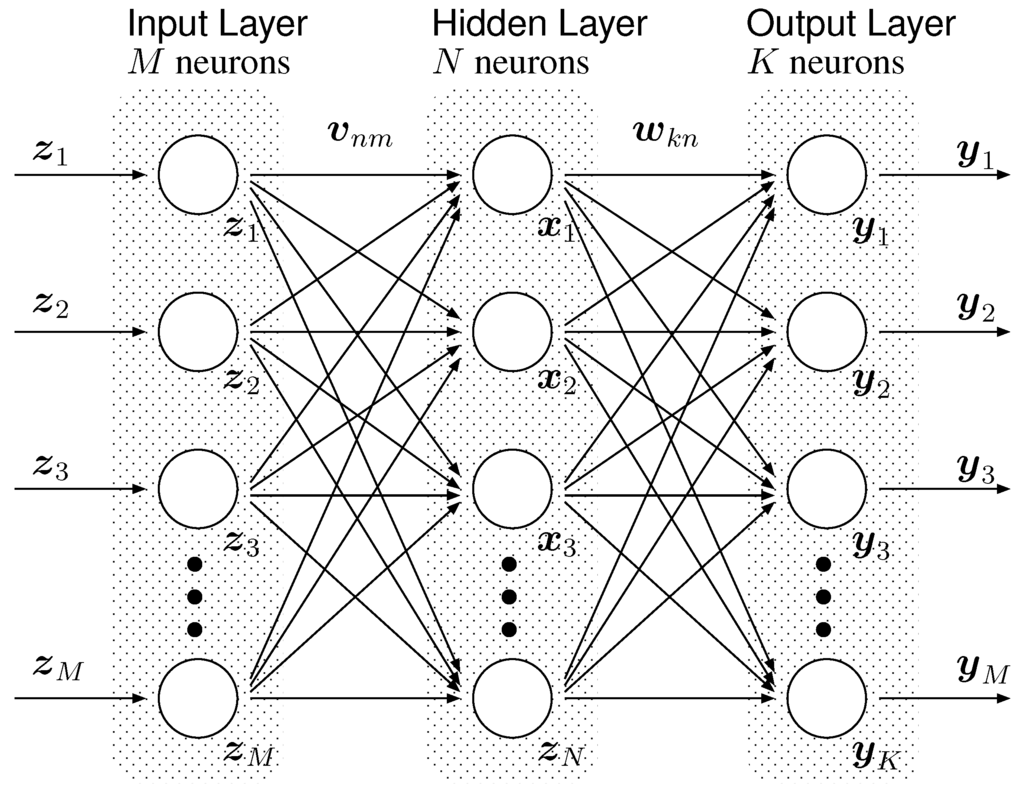
\includegraphics[width=0.45\textwidth]{figures/multilayer_perceptron.png}
    \caption{A multilayer perceptron neural network with 1 hidden layer.
        Figure courtesy of Teijiro Isokawa, Haruhiko Nishimura and Nobuyuki Matsui.}
    \label{Fig:MLPArchitecture}
\end{figure}

\subsection{Restricted Boltzmann Machine}
Restricted Boltzmann machine (RBM)~\cite{RBMTechReport} is a type of energy-based model,
which associate a scalar energy to each configuration vector of the variables in the network.
In energy-based model, learning is the process of configuring the network weights so that
the average energy over training data is minimized.
RBM consists of a layer of hidden units (H) and a layer of visible units (V).
Here ``restricted" means that connections are just between hidden and visible layer,
but not within hidden layers or visible layers.
This makes its training to be faster than Boltzmann machine and makes it feasible to
stack multiple separately trained RBM together to form deep architecture.
A joint configuration, $(\mathbf{v, h})$, of the visible and hidden units has the energy of
\begin{align}
    E(\mathbf{v, h}) &= -\sum_{i\in visible}a_i v_i - \sum_{j\in hidden}b_j h_j - \sum_{i, j}v_i h_j w_{ij}
\end{align}
where $a=\{a_i\}$ and $b=\{b_j\}$ are biases in visible and hidden layer respectively,
and $W=\{w_{ij}\}$ is the weights between them.
The network assigns a probability to every possible pair of $(\mathbf{v, h})$ via this energy
function
\begin{align}
    p(\mathbf{v, h}) &= \frac{1}{Z} e^{-E(\mathbf{v, h})} \\
    p(\mathbf{v}) &= \frac{1}{Z} \sum_{\mathbf{h}} e^{-E(\mathbf{v, h})}
\end{align}
where $Z$ is the partition function that equals to the summation over all possible hidden
and visible vector pairs
\begin{align}
    Z = \sum_{\mathbf{v,h}} e^{-E(\mathbf{v, h})}
\end{align}
Based on the ``maximizing log likelihood" idea,
we want to raise the probability of a training example and it can be done by
adjusting the weights biases to lower the energy of the considered example.
Meanwhile, we can let other examples make a big contribution to the partition function $Z$
by raising their energy.
Both insights can be translated to the following formula:
\begin{align}
    \frac{\partial \log p(v)}{\partial w_{ij}} = \langle v_i h_j \rangle_{data} - \langle v_i h_j \rangle_{model} 
\end{align}
This implies the following learning rule for performing stochastic gradient ascent on training
data
\begin{align}
    \Delta w_{ij} &= \varepsilon (\langle v_i h_j \rangle_{data} - \langle v_i h_j \rangle_{model})
\end{align}
The first term $\langle v_i h_j \rangle_{data}$ is the sampling from the data and it is easy to
compute since there is no directed connection between hidden units.
The sampling of $h_j$ is based on the probability
\begin{align}
    Prob(h_j = 1 | \mathbf{v}) &= sigmoid(b_j + \sum_i{v_i w_{ij}})
    \label{Equ:RBMSampleHidden}
\end{align}
Similarly, $v_i$ can be sampled with the following distribution
\begin{align}
    Prob(v_i = 1 | \mathbf{h}) &= sigmoid(a_j + \sum_j{h_i w_{ij}})
    \label{Equ:RBMSampleVisible}
\end{align}
The term $\langle v_i h_j \rangle_{model}$ can be obtained by performing alternative Gibbs
sampling for a long time.
The sampling starts from a random visible state.
Then we update the hidden units in parallel with Equation~\ref{Equ:RBMSampleHidden},
followed by updating the visible units in parallel with Equation~\ref{Equ:RBMSampleVisible}.
Instead of doing alternating Gibbs sampling for a large number of iterations,
\cite{TrainCD} proposed contrastive divergence (CD) as a faster learning procedure.
The training also start with a training vector to compute the states of the hidden units
using Equation~\ref{Equ:RBMSampleHidden}.
Then, with the chosen hidden states, we reconstruct the visible states by sampling each $v_i$
with probability given in Equation~\ref{Equ:RBMSampleVisible}.
The change of weight is then computed by
\begin{align}
    \Delta w_{ij} = \varepsilon (\langle v_i h_j \rangle_{data} -
    \langle v_i h_j \rangle_{reconstruct})
    \label{Equ:RBMCD1}
\end{align}
This is called contrastive divergence using one full step of alternating Gibbs sampling.
Contrastive divergence with $n$ rounds of alternating Gibbs sampling
is usually denoted as CD$n$.

The layer-by-layer training algorithm for stacking RBMs goes in a greedy fashion.
After learning the first layer RBM, the activity vector of the hidden units can be used
as ``data" for training the RBM in the second layer
and this process can be repeated to learn as many hidden layers as desired.
As data passing through the RBMs, we obtain the highest level features 
which are typically fed into a classifier.
The entire deep network (RBMs plus the classifier) can be fine-tuned to
improve the classification performance.


\begin{figure}[h]
    \centering
    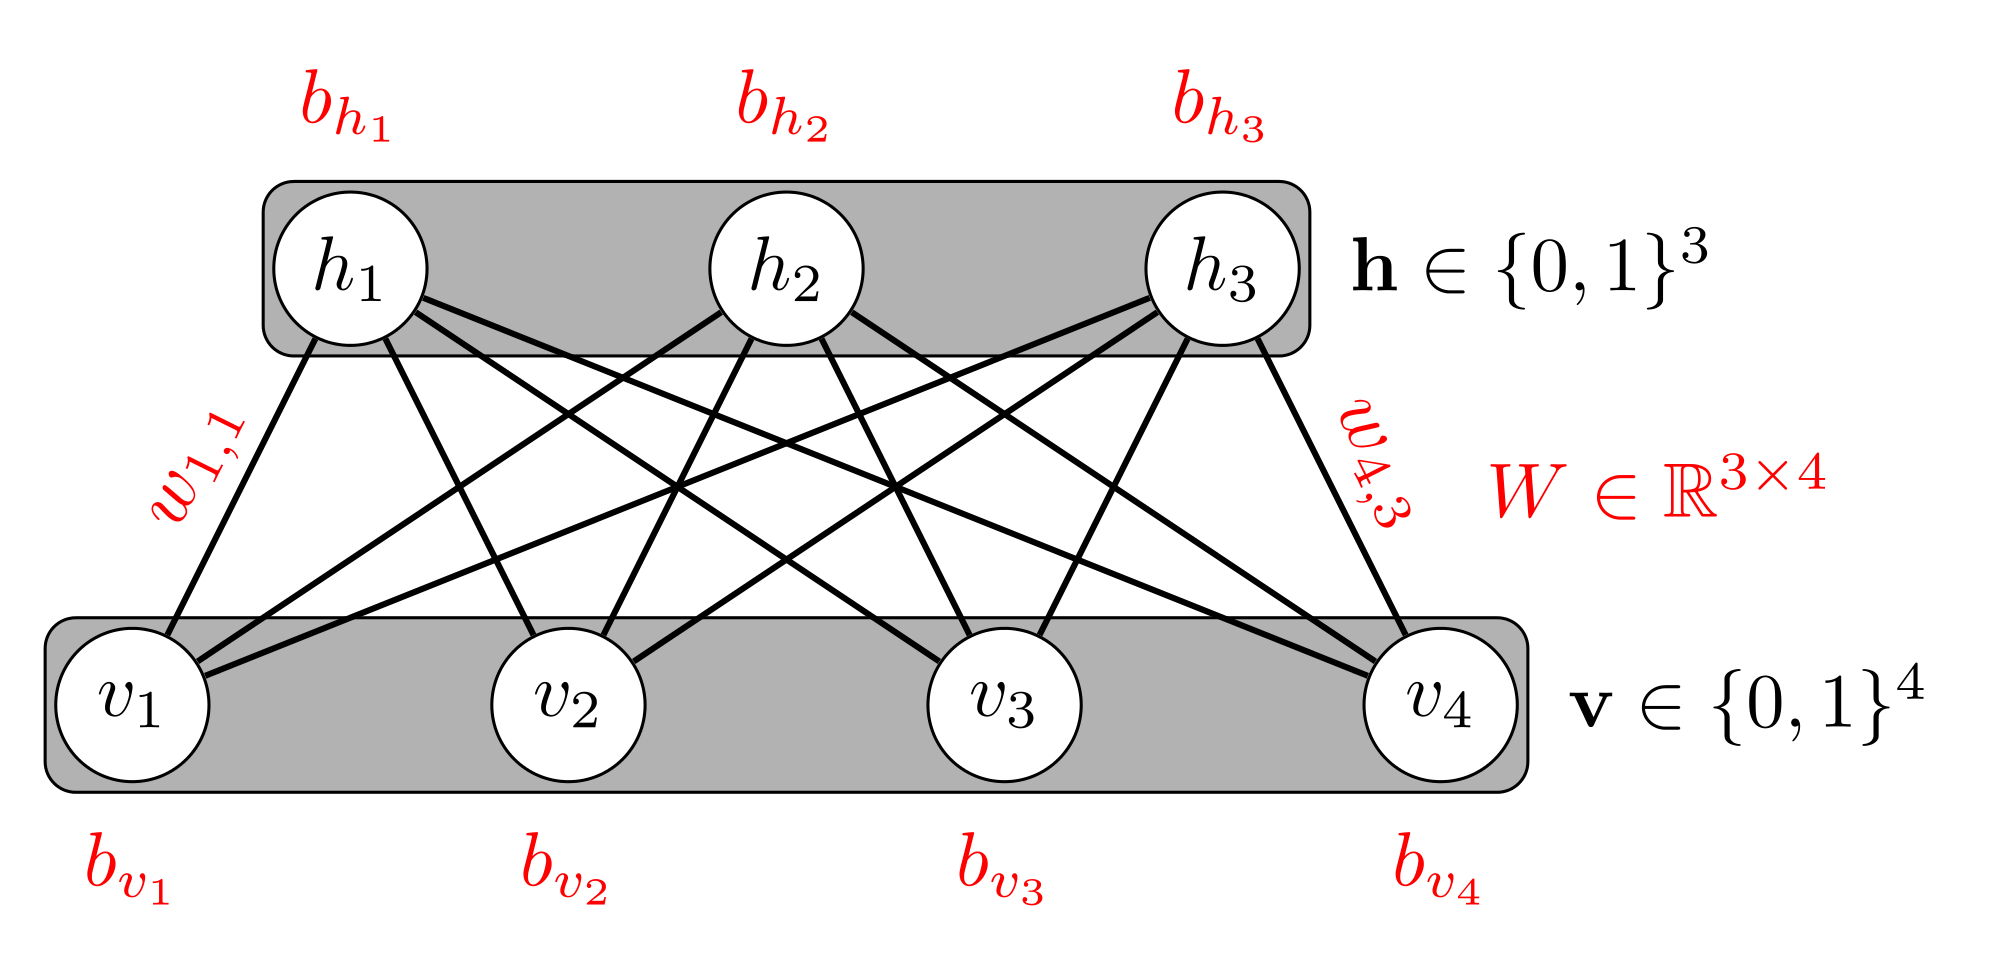
\includegraphics[width=0.45\textwidth]{figures/rbm.png}
    \caption{Restricted Boltzmann Machine.
        Figure courtesy of https://commons.wikimedia.org/wiki/File:Restricted-boltzmann-machine.svg}
    \label{Fig:RBMArchitecture}
\end{figure}



\subsection{Autoencoders}
An autoencoder neural network is an unsupervised model with typically one hidden layer that
tries to set the output layer to be equal to the input.
As shown in Figure~\ref{Fig:AEArchitecture}, we want the network to
learn a function $h_{W, b}(x) \approx x$.
However, to prevent the network from learning the meaningless identity function,
we need to place extra constraints on the network, giving birth to different
flavors of autoencoders.
In this project we consider two most popular types of autoencoder, sparse autoencoder and
denoising autoencoder.

The \textbf{denoising autoencoder} algorithm is proposed by~\cite{DenoiseAE} and illustrated in
Figure~\ref{Fig:dAEAlgorithm}.
To prevent learning identity function, an example $\mathbf{x}$ is first corrupted, either by
adding Gaussian noise or by random masking a fraction of items in $\mathbf{x}$ to zero.
The autoencoder then maps corrupted $\mathbf{\tilde{x}}$ to a hidden representation $\mathbf{y} = sigmoid(\mathbf{W}\tilde{\mathbf{x}} + \mathbf{b})$.
From $\mathbf{y}$ we reconstruct $\mathbf{z}=g_\theta'(\mathbf{y})$.
The training needs to learn the parameters $\theta$ and $\theta'$ so that
average reconstruction error is minimized over training set.
For binary input $\mathbf{x}$, usually cross entropy is adopted as $L_H(\mathbf{x}, \mathbf{z})$;
while mean squared error is used for real-valued $\mathbf{x}$.

\begin{figure}[h]
    \centering
    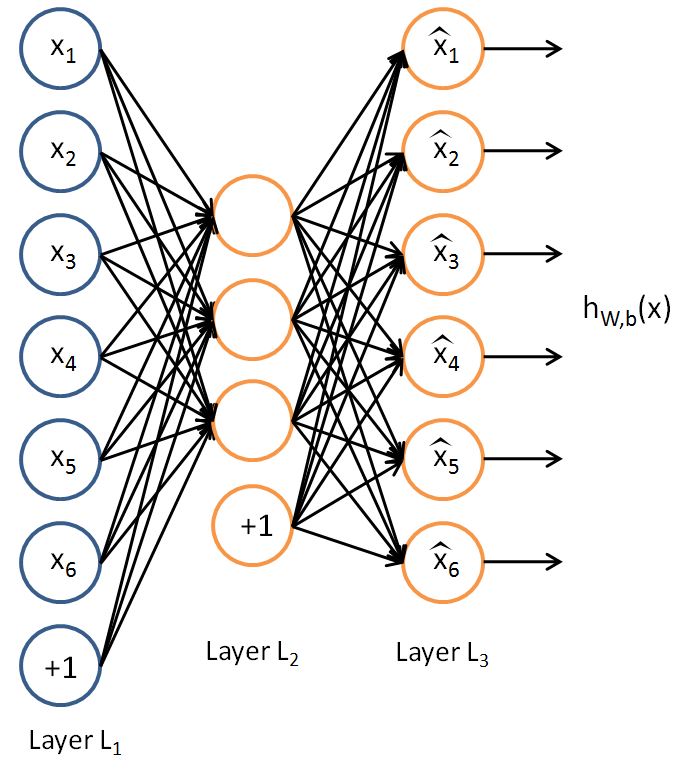
\includegraphics[width=0.45\textwidth]{figures/autoencoder.png}
    \caption{General Architecture of Autoencoders.
        Figure courtesy of~\cite{UFLDLAutoencoder}.}
    \label{Fig:AEArchitecture}
\end{figure}

\begin{figure}[h]
    \centering
    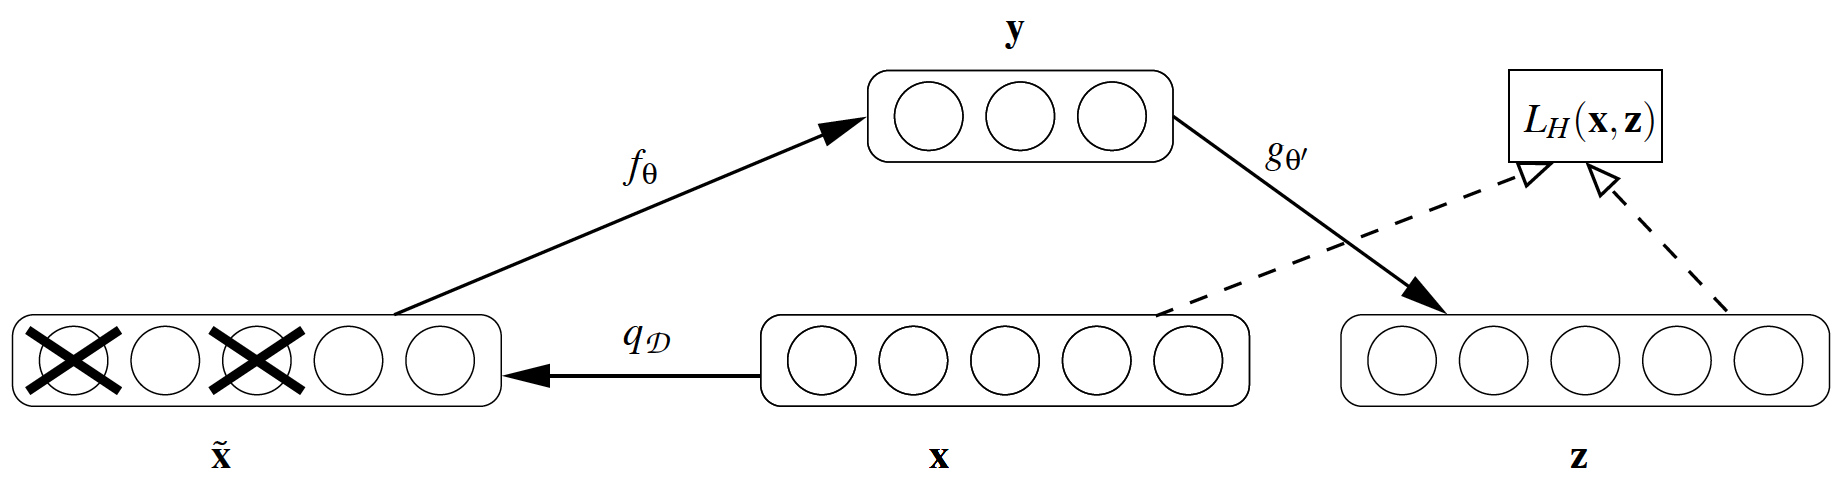
\includegraphics[width=0.45\textwidth]{figures/denoiseautoencoder.png}
        \caption{The denoising autoencoder algorithm.
        Input example $\mathbf{x}$ is randomly corrupted via $q_\mathcal{D}$ and then
        is mapped via encoder $f_\theta$ to $\mathbf{y}$.
        The decoder $g_\theta'$ attempts to reconstruct $\mathbf{x}$ and produces $\mathbf{z}$.
        Reconstruction error is measured by loss $L_H(\mathbf{x}, \mathbf{z})$, to be minimized
        during the training phase.
        Figure courtesy of~\cite{DenoiseAE}.}
    \label{Fig:dAEAlgorithm}
\end{figure}

The \textbf{sparse autoencoder} works by placing a sparsity constraint on the hidden units~\cite{SparseAE}.
First, we make the autoencoder's hidden layer size to be over-complete,
that is, of larger size comparing to the dimension of the input.
Let's denote the activation of hidden unit $j$ of layer 2 in Figure~\ref{Fig:AEArchitecture}
to be $a^2_j(\mathbf{x})$ given input example $\mathbf{x}$.
With that, we define the average activation of hidden unit $j$ over the $m$-size
training set
\begin{align}
    \hat{\rho}_j = \frac{1}{m} \sum_{i=1}^{m} a^2_j(\mathbf{x})
\end{align}
The sparsity constraint is enforcing, $\forall$ hidden unit $j$,
\begin{align}
    \hat{\rho}_j = \rho
\end{align}
where $\rho$ is a sparsity parameter that approximates zero (say 0.05).
This constraint can be vectorized over the hidden layer, say of size $n_2$,
with the KL divergence based penalty term
\begin{align}
    \sum_j^{n_2} KL(\rho || \hat{\rho}_j)
    = \sum_j^{n_2} [\rho \log \frac{\rho}{\hat{\rho}_j} + (1 - \rho) \log \frac{1-\rho}{1-\hat{\rho}_j} ]
\end{align}
The sparsity penalty term is integrated into the cost function by adding another hyper-parameter $\beta$
\begin{align}
    L(W, b) = \frac{1}{2}||h_{W,b}(\mathbf{x}) - \mathbf{x}||^2 +
    \beta \sum_j^{n_2} KL(\rho || \hat{\rho}_j)
\end{align}

Denoising autoencoder and sparse autoencoder, surprisingly, have different application domains.
Vincent et al.~\cite{DenoiseAE} have shown that stacked denoising autoencoder can be used to
initialize a deep neural network's weight parameter,
achieving similar and sometimes better performance than stacked RBM.
They also show that training stacked denoising autoencoder with MNIST dataset, it is able
to re-synthesize a variety of similarly good quality digits.
Raina et al.~\cite{SparseAE} have compared sparse encoding with principle component analysis
(PCA) and argue that transferring raw features with a well unsupervised trained
sparse autoencoder can be beneficial to supervised learning algorithms,
for example support vector machines (SVM).


\subsection{Generative Adversarial Nets}
As another generative model, Generative Adversarial Nets (GAN)\cite{GAN} adopts a novel training framework,
in which two models are trained simultaneously and adversarially.
The generative model $G(z;\theta_g)$ aims to capture the probability distribution of the available unlabelled dataset,
where its input is a noise variable $z$ following a prior distribution $p_z$.
The discriminative model $D(x;\theta_d)$ output the probability that whether the its input source $S$ comes
from training dataset ($x\sim data$) or the generative model ($x \sim G(z)$):
\begin{align}
    D(X) = P(S|X)
\end{align}

Models $G$ and $D$ can be as simple as multilayer perceptrons,
or as complex as deep convolutional nets when training dataset is images.
The two models are trained in opposition to one another, with respect to the log-likelihood
function
\begin{equation}
\begin{aligned}
V(D, G) = & \mathbb{E}_{\bm{x}\sim data} [\log P(S=real|X=\bm{x})] + \\
          & \mathbb{E}_{\bm{x}\sim G(\bm{z})} [\log P(S=fake|X=\bm{x})] \\
        = & \mathbb{E}[\log D(\bm{x})] + \mathbb{E}[\log (1 - D(G(\bm{z})))]
\end{aligned}
\end{equation}
With $V(D, G)$ properly defined, the training procedure is a two-player minimax game.
First we make $D$ maximize the log-likelihood that it correctly recognize
both the training examples and samples generated from $G$;
at the same time, we make $G$ to generate samples that trick $D$ to make mistake about the
generated samples.
This two-phase min-max optimization can be summarized as:
\begin{align}
    \min_G \max_D V(D, G)
\end{align}

Powerful though GAN is, large amount of efforts are needed in training.
One way to make the training stable and fast is to augment an auxiliary classifier so that
the training phase can employ the labels if available in the dataset~\cite{AC-GAN}.
In auxiliary classifier GAN (AC-GAN), the discriminator $D$ now gives both a probability
distribution over the sources (whether $\bm{x}$ is real or fake) and a probability distribution
over the class labels:
\begin{align}
    D(X) = P(S|X), P(C|X)
\end{align}
Accordingly, the log-likelihood function $V(D, G)$ is augmented with the log-likelihood of the correct class:
\begin{equation}
\begin{aligned} 
    V(D, G) &= L_S + L_C \\
    L_S = & \mathbb{E}_{\bm{x} \sim data} [\log P(S=real|X=\bm{x})] + \\
          & \mathbb{E}_{\bm{x} \sim G(\bm{z})} [\log P(S=fake|X=\bm{x})] \\
    L_C = & \mathbb{E}_{\bm{x} \sim data}[\log P(C=c|X=\bm{x})] + \\
          & \mathbb{E}_{\bm{x} \sim G(\bm{z})} [\log P(C=c|X=\bm{x})]
\end{aligned}
\end{equation}
The training procedure for AC-GAN is similar to GAN: we train $D$ to maximize $V(D, G)$;
while at the same time we train $G$ to minimize $L_S - L_C$.


\subsection{Wide and Deep Learning with Embeddings}

